% Intended LaTeX compiler: pdflatex
\documentclass[final,anonym]{mcarticle}
% org-mc-latex.el ----------------------
\usepackage[utf8]{inputenc}
% extra (#+LaTeX_HEADER: lines) --------

% end of `org-latex-classes' -------------------------------------------------
\author{Fabrice Niessen}
\date{\today}
\title{Fichier de démo}
\hypersetup{
 pdfauthor={Fabrice Niessen},
 pdftitle={Fichier de démo},
 pdfkeywords={},
 pdfsubject={},
 pdfcreator={Emacs 26.1 (Org mode 9.1.9)}, 
 pdflang={Frenchb}}
\begin{document}

\maketitle

\section{Contexte}
\label{sec:orge64a0d9}

Lorem ipsum dolor sit amet, consectetur adipisicing elit, sed do eiusmod
tempor incididunt ut labore et dolore magna aliqua. Ut enim ad minim veniam,

\begin{center}
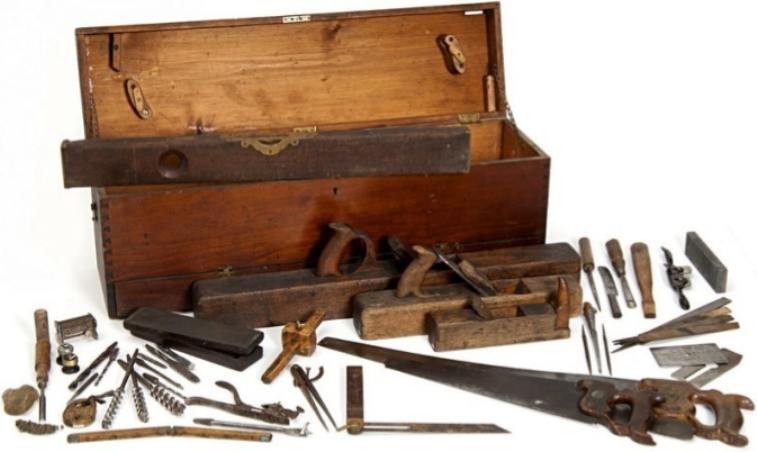
\includegraphics[width=.75\linewidth]{images/toolbox-messy.png}
\end{center}

\section{Explications}
\label{sec:org1f4241f}

quis nostrud exercitation ullamco laboris nisi ut aliquip ex ea commodo
consequat. Duis aute irure dolor in reprehenderit in voluptate velit esse

\begin{table}[!htbp]
\caption{\label{tab:org5bf5c53}
Montants}
\centering
\begin{tabular}{lr}
Mois & Montant\\
\hline
resto & 25\\
cinema & 12\\
babysit & 21\\
\end{tabular}
\end{table}

\begin{center}
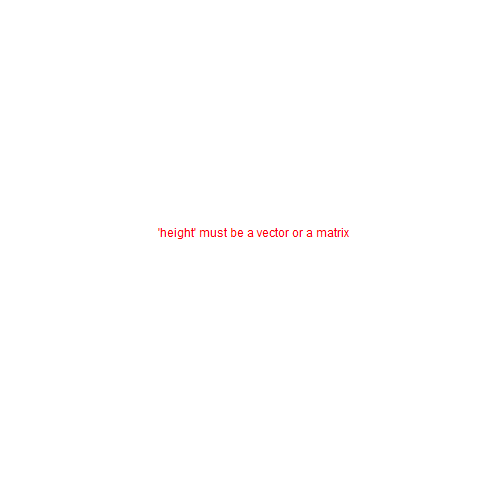
\includegraphics[width=.75\linewidth]{images/Rplots.png}
\end{center}

\section{Conclusions}
\label{sec:orgac49de5}

cillum dolore eu fugiat nulla pariatur. Excepteur sint occaecat cupidatat non
proident, sunt in culpa qui officia deserunt mollit anim id est laborum.
\end{document}
